\documentclass[12pt, french]{article}

\usepackage{fancyhdr, fancybox, lastpage,mhchem, mathrsfs, tikz}
\usepackage[most]{tcolorbox}
\usepackage[a4paper, margin={0.3in, .75in}]{geometry}
\usepackage{wrapfig}
\pagestyle{fancy}
\renewcommand\headrulewidth{1pt}
\renewcommand\footrulewidth{1pt}
\fancyhf{}
\rhead{ \em{Zakaria Haouzan}}
\lhead[C]{\em{2ème année baccalauréat Sciences Physiques}}
\chead[C]{}
\rfoot[C]{}
\lfoot[R]{}
\cfoot[]{\em{Page \thepage / \pageref{LastPage}}}


\newtcolorbox{Box2}[2][
enhanced, 
    breakable,
]{
                lower separated=false,
                colback=white,
colframe=white!20!black,fonttitle=\bfseries,
colbacktitle=white!30!gray,
coltitle=black,
enhanced,
attach boxed title to top left={yshift=-0.1in,xshift=0.15in},
title=#2,#1}


\begin{document}
\begin{center}
   \shadowbox {\bf{Mouvement d'une particule chargée dans un champ
magnétique uniforme}
 }

\end{center}

\vspace{-0.2cm}
%%_________________________Exercice ! :"_________________________Exercice
   \begin{Box2}{Exercice 1 : Mouvement d'une particule chargée dans un champ
magnétique uniforme}

	\begin{wrapfigure}[4]{r}{0.26\textwidth}
  \begin{center}
	  \vspace{-0.6cm}
	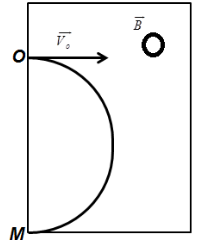
\includegraphics[width=0.26\textwidth]{./ex_00.png}
  \end{center}
\end{wrapfigure}

Les ions $Mg^{2+}$ pénètrent dans une région de l'espace où règne un champ $\vec{B}$(perpendiculaire au plan de la figure). Avec une vitesse
magnétique uniforme  $V_0 =1,6.10^4.m.s^{-1}$
\begin{enumerate}


	\item  Donner les caractéristiques de la force magnétique $\vec{F_m}$.
	\item  Déterminer le sens du champs magnétique $\vec{B}$.
	\item  En appliquant la deuxième loi de newton dans un référentiel galiléen,
		montrer que le mouvement des ions $Mg^{2+}$ est circulaire uniforme.
	\item  Calcule la masse d'ion $Mg^{2+}$ (On donne $OM = 4 cm$ )

\end{enumerate}

\textbf{Données :} L'intensité du champs magnétique $B= 0,1T$ ; La charge élémentaire $e = 1, 6.10^{-19} C$


   \end{Box2}


%%_________________________Exercice !2 :"_________________________Exercice
\begin{Box2}{Exercice 2 :Les isotopes }
	\begin{wrapfigure}[1]{r}{0.32\textwidth}
  \begin{center}
	  \vspace{-0.6cm}
	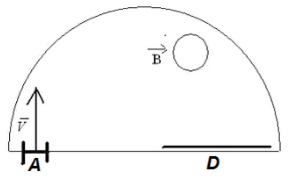
\includegraphics[width=0.32\textwidth]{./ex_01.png}
  \end{center}
\end{wrapfigure}


	On considère les ions de deux isotopes $^{200}_{80}Hg^{2+}$ et $^{202}_{80}Hg^{2+}$ du mercure.

Ils pénètrent en $A$, avec une vitesse $V$ non nulle, dans une capsule où \\règne un champ magnétique uniforme
\\(perpendiculaire au plan de la feuille):
\begin{enumerate}

	\item Indiquer le sens du champ magnétique pour que les ions soient\\
déviés vers le détecteur $D$.
\item Montrer que dans cette capsule les ions ont un mouvement
uniforme, et exprimer les rayons $R$ de la trajectoire de deux
isotopes en fonction de $m$, $e$, $v$ et $B$.
\item Déterminer lequel de ces deux ions va être le plus dévié.
Justifier.
\end{enumerate}
\end{Box2}

\begin{Box2}{Exercice 3 :Etude du mouvement d’une particule chargée dans un champ magnétique  }
	Deux particules chargées $Li^+$ et $X^{2+}$ sont introduites en un point O, avec la même vitesse
	initiale $\vec{V}$ , dans un espace où règne un champ magnétique uniforme $\vec{B}$ , perpendiculaire au
	vecteur $\vec{V}$.

	$q_X$ et $m_X$ sont respectivement la charge électrique et la masse de la particule $X^{2+}$.
	On considère que $Li^+$ et $X^{2+}$ sont soumises
seulement à la force de Lorentz.

\textbf{Données : }
\begin{itemize}
\item La vitesse initiale : $V=10^5 m.s^{-1}$ ;
\item L’intensité du champ magnétique : $B= 0,5T$ ;
\item La charge élémentaire: $e =1,6.10^{-19} C$;
\item La masse de $Li^+$ : $m_Li = 6,015u$ ;
\item $1u=1,66.10^{-27} kg$ ;
\item La figure 1 représente les trajectoires des deux particules dans le champ $\vec{B}$
\item On rappelle l’expression de la force de Lorentz : $\vec{F} = q\vec{v} \wedge \vec{B}$.
\end{itemize}
 
\begin{center}
	  \vspace{-0.6cm}
	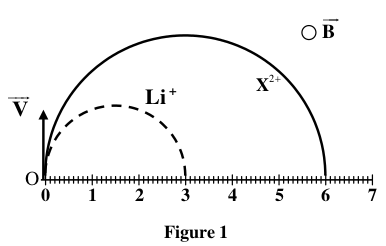
\includegraphics[width=0.42\textwidth]{./ex_02.png}
  \end{center}

  \begin{enumerate}
	\item Déterminer la direction, le sens et l’intensité du vecteur force de Lorentz exercée sur la particule $Li^+$ au point O.


	\item Préciser le sens du vecteur $\vec{B}$ en le représentant par $\bigodot$ s’il est vers l’avant ou par $\bigoplus$ s’il est vers l’arrière.

	\item En appliquant la deuxième loi de Newton dans un référentiel galiléen, montrer que le mouvement de l’ion $Li^+$ est uniforme et de trajectoire circulaire de rayon $$R_{Li^+} = \frac{m_{Li^+}.V}{e.B}$$

\item En exploitant les données de la figure 1, déterminer le rapport $\frac{R_{X^{2+}}}{R_{Li^+}}$ ;

		avec $R_{X^{2+}}$ le rayon de la trajectoire de la particule $X^{2+}$.

	\item Sachant que la particule $X^{2+}$ se trouve parmi les trois ions proposés avec leurs masses dans le
		tableau ci-dessous, identifier $X^{2+}$ en justifiant la réponse.


\end{enumerate}
\begin{center}
\begin{tabular}{ |c|| c| c|c| }
	\hline
	Ion & $^{24}_{12}Mg^{2+}$ &$^{16}_{12}Mg^{2+}$ &$^{40}_{20}Ca^{2+}$ \\\hline
	Masse(u) & 23,985 & 25,983 &39,952 \\\hline
\end{tabular}
\end{center}
\end{Box2}
	%\vspace{-0.8cm}


%\begin{Box2}{Exercice 4 :Les toboggans}

%\end{Box2}




%\begin{Box2}{Exercice 5 : Etude du mouvement du centre de gravité d’une balle. }
%%\begin{wrapfigure}[3]{r}{0.33\textwidth}
	%%\vspace{-0.8cm}

%\end{Box2}


%\begin{center}
   %\Large{ \em{Exercices Supplémentaires}}
%\end{center}

%\vspace{-0.8cm}

%%%_________________________Exercice ! 3:"_________________________Exercice
%\begin{Box2}{Exercice 6:Etude du mouvement d’une balle de golf dans le champ de pesanteur uniforme }
%%\begin{wrapfigure}{r}{0.4\textwidth}
 %%\end{wrapfigure}

%\end{Box2}

%%_________________________Exercice 4 : _________________________Exercice
%\begin{Box2}{Exercice 7 :Le ski }
   %% \begin{wrapfigure}[12]{r}{0.5\textwidth}

%%\end{wrapfigure}


%\end{Box2}
\begin{center} \emph{\textbf{““Winning doesn't always mean being first. ...”}}
\end{center}

%\vspace{-0.6cm}
%%%_________________________Exercice 5 : _________________________Exercice
%\begin{Box2}{Exercice 4 : }
   %% \begin{wrapfigure}[14]{r}{0.5\textwidth}
  %%\begin{center}
	  %%\vspace{-0.6cm}
	%%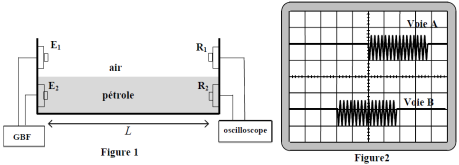
\includegraphics[width=0.5\textwidth]{./img/ex5.png}
  %%\end{center}
%%\end{wrapfigure}

%4

%\end{Box2}

%\begin{Box2}{Exercice 5 : }

%44
%\end{Box2}


%\begin{Box2}{Exercice 6 : }


	%\end{Box2}


%\begin{Box2}{Exercice 7 : }
%\end{Box2}
\end{document}
